\section{Approach} \label{sec:approach}
This section describes our approach and gives an insight of the process supporting it. In the first step, we show how performance improvement can be achieved by
reducing the number of access control rules that have to be considered at the evaluation time, through the definition of policy based splitting criteria. 
Secondly, we show how to select the splitting criterion that preserves the synergy requirement in the access control architecture.

\subsection{XACML Policy Refactoring Process}
What happens in a request evaluation process is that for a given access control request, some rules are evaluated in the global policy whereas some of those rules are not
 applicable to the request. Starting from this observation, we propose to evaluate only the relevant rules for a given request in the decision making process. 
We propose to split the initial policy into smaller policies based on attribute values combination. We transform the policy \normalsize $P$ into smaller 
policies \normalsize $P_{SC_{w}}$ where each policy conforms to a Splitting Criteria $SC_{w}$. An $SC_{w}$ defines the set of attributes that are considered 
to classify all the rules into subsets having the same attribute values where $w$ denotes the number of attributes that have to be considered conjointly for aggregating 
rules into a unified set based on specific attribute elements selection. A policy can be split into a set of policies where the rules have the same subject, resource, or action. 
Rules can also be aggregated considering two attributes like $<Subject, Action>$ or $<Action, Resource>$, in this setting, a policy will be transformed into a set of smaller 
policies where rules in the resulting policies have the same couple of attribute elements. We can go further in our grouping strategy when using $P_{SC_{w}}$ whose 
rules match a specific triplet of resource, action and subject. Table I shows all splitting criteria categories according to the attribute elements combination.
\begin{table}[h!]
\centering
\setlength{\extrarowheight}{6 pt}
\begin{tabular}{|>{\small}c|>{\small}c|} 
\hline  \rowcolor{black} 
 \bf
\textcolor{white}{Categories}& \bf \textcolor{white}{Splitting Criteria}\\ \hline
 $SC_{1}$& {$<Subject>, <Resource>, <Action>$}\\ \hline

$SC_{2}$& {$<Subject,Action>, <Subject,Resource>$}\\&{$<Resource,Action>$}\\  \hline

$SC_{3}$& {$<Subject,Resource,Action>$}\\ \hline
\end{tabular}
\caption{Splitting Criteria}
\label{table1}\end{table}
Once the splitting process is performed, the access control architecture will include one or more (PDPs) that comply with a certain splitting criterion.
 
\subsection{Architecture Model Preservation: PEP-PDP Synergy}
We consider the different splitting criteria that we have identified in the previous section and we propose to select the splitting criterion that 
enables to preserve the synergy requirement in the access control architecture. This splitting criterion respects how PEPs are organized 
at the application level and how they are linked to their corresponding PDPs.
A deep analysis of the PEPs at the application enables to observe the mapping between the PEPs and the PDP. At the application level, the PEP
is represented by a method call that triggers a decision making process by activating some specific rules in the PDP.
The code below is taken from \cite{legacy}, this code excerpt shows an example of a PEP represented by the method checkSecurity which calls the class 
SecurityPolicyService that initiates the PDP component.
\begin{algorithmic}
\begin{algorithm}[!h]
   \STATE public void borrowBook(User user, Book book)
   \STATE throws SecuritPolicyViolationException {
   \STATE   // call to the security service
\STATE \hspace{0.5cm} \textbf{ServiceUtils.checkSecurity(user,
\STATE LibrarySecurityModel.BORROWBOOK\_METHOD,
\STATE LibrarySecurityModel.BOOK\_VIEW);
\STATE ContextManager.getTemporalContext());}
    \STATE  // call to business objects
    \STATE  // borrow the book for the user
\STATE \hspace{0.5cm} book.execute(Book.BORROW, user);
\STATE      // call the dao class to update the DB
\STATE \hspace{0.5cm} bookDAO.insertBorrow(userDTO, bookDTO);}
\end{algorithm}
\end{algorithmic}

An analysis of this code reflects that the PEP presented by the method ServiceUtils.checkSecurity will trigger exclusively all the rules 
that have the subject user (provided as input parameter in the PEP) and fixed Action (LibrarySecurityModel.BORROWBOOK\_METHOD) and Resource ( LibrarySecurityModel.BOOK\_VIEW).
Thus the splitting process that will preserve the mapping between the PEPs and the PDP will be $SC_{2}=<Resource,Action>$ in this case since the rules in the policy are triggered 
by Action, Resource. Depending on the application, establishing this mapping may require to identify all the enforcements points in the application, and to 
track the different method calls triggered from these specific enforcement calls to map them to the relevant access control rules.
In the worst case, splitting the initial PDP into multi-PDPs may lead to a non-synergic system: a PEP may send its requests to several PDPs. 
The PDP, which receives a request is only known at runtime. Such a resulting architecture breaks the PEP-PDP synergy and the conceptual 
simplicity of the initial architecture model. 
In the best case, the refactoring preserves the simplicity of the initial architecture, by keeping a many-to-one association from PEPs to PDPs. A given request evaluation 
triggered by one PEP will always be handled by the same PDP. Operationally, the request evaluation process will involve 
one XACML policy file. In this case, the refactoring is valid, since its does not impact the conceptual architecture of the system.
Our empirical results, presented in section~\ref{sec:experiment}, have shown that adopting a policy refactoring based on system functions, as a refactoring strategy, enables to 
have the best splitting criterion in term of performance. 
As depicted in Figure \ref{overallprocess}, the refactoring process is automated and starts by specifying and creating the XACML file which 
will be split by our tool according to a specified SC that can be chosen by an access control stakeholder. Afterwards, the policies are included in the 
framework that supports our approach. For every change in the access control policy, the initial policy is updated and 
split again in order to be included again in the framework.
From a point of view of the system administration, maintaining and updating the access control policies is completely a standalone and simple
 process. The input is usually a centralized XACML policy. This input remains the same than before the access control performance issue is tackled.
Our process is transparent in the sense that it does not impact the existing functional aspects of the access control management system, 
for system administrators, who have to update the policy fequently and have to manage various dimensions of access control 
systems such the scalability and maintainability.
\begin{figure}[!h]
\begin{center}
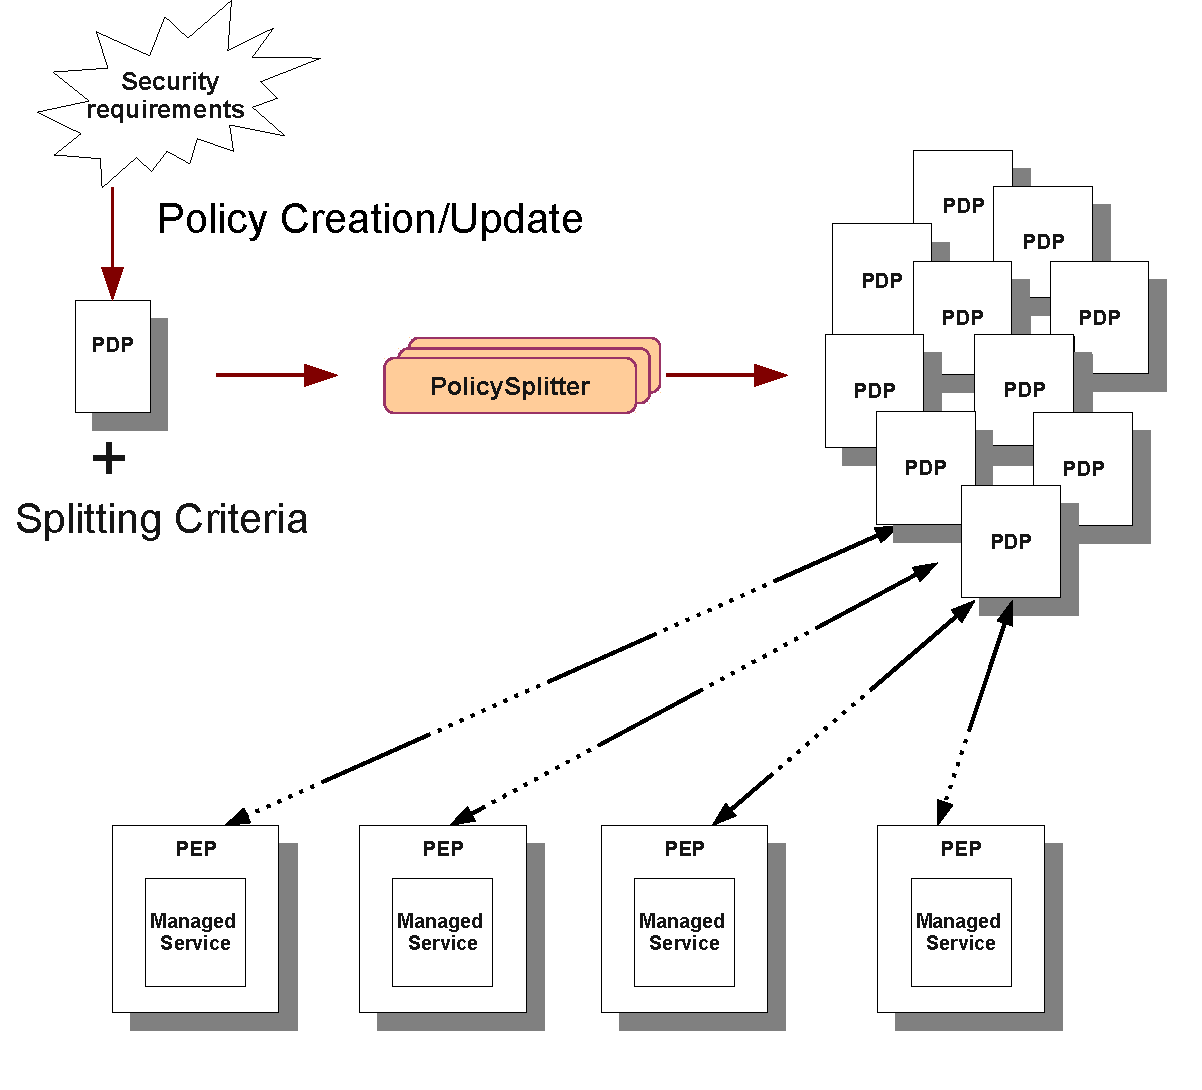
\includegraphics[width=8.5cm, height=8cm]{Overall-process}

\caption{Overview of the process of defining and deploying Access Control Policies}

\label{overallprocess}

\end{center}

\end{figure} 